\documentclass[english, 11 pt, class=article, crop=false]{standalone}
%\documentclass[english, 11 pt]{report}
\usepackage[T1]{fontenc}
\usepackage[utf8]{luainputenc}
\usepackage{babel}
\usepackage[hidelinks, bookmarks]{hyperref}
\usepackage{geometry}
\geometry{verbose,tmargin=1cm,bmargin=3cm,lmargin=4cm,rmargin=4cm,headheight=3cm,headsep=1cm,footskip=1cm}
\setlength{\parindent}{0bp}
\usepackage{amsmath}
\usepackage{amssymb}
\usepackage{esint}
\usepackage{import}
\usepackage[subpreambles=false]{standalone}
%\makeatletter
\addto\captionsenglish{\renewcommand{\chaptername}{Kapittel}}
\makeatother
\usepackage{tocloft}
\addto\captionsenglish{\renewcommand{\contentsname}{Innhold}}
\usepackage{graphicx}
\usepackage{placeins}
\raggedbottom
\usepackage{calc}
\usepackage{cancel}
\makeatletter
\usepackage{color}
\definecolor{shadecolor}{rgb}{0.105469, 0.613281, 1}
\usepackage{framed}
\usepackage{wrapfig}
\usepackage{bm}
\usepackage{ntheorem}

\usepackage{ragged2e}
\RaggedRight
\raggedbottom
\frenchspacing

\newcounter{lign}[section]
\newenvironment{lign}[1][]{\Large \refstepcounter{lign} \large
	\textbf{\thelign #1} \rmfamily}{\par\medskip}
\numberwithin{lign}{section}
\numberwithin{equation}{section}
\usepackage{xcolor}
\usepackage{icomma}
\usepackage{mathtools}
\usepackage{lmodern} % load a font with all the characters
\usepackage{xr-hyper}
\makeatother
\usepackage[many]{tcolorbox}

%\setlength{\parskip}{\medskipamount}
\newcommand{\parskiplength}{11pt}
%\setlength{\parskip}{0 pt}
\newcommand\eks[2][]{\begin{tcolorbox}[enhanced jigsaw,boxrule=0.3 mm, arc=0mm,breakable,colback=green!30] {\large \textbf{Eksempel #1} \vspace{\parskiplength}\\} #2 \vspace{1pt} \end{tcolorbox}\vspace{1pt}}

\newcommand\fref[2][]{\hyperref[#2]{\textsl{Figur \ref*{#2}#1}}}
\newcommand{\hr}[2]{\hyperref[#2]{\color{blue}\textsl{#1}}}

\newcommand\rgg[2][]{\begin{tcolorbox}[boxrule=0.3 mm, arc=0mm,colback=orange!55] #2 \vspace{1pt} \end{tcolorbox}\vspace{-2pt}}
\newcommand\alg[1]{\begin{align*} #1 \end{align*}}
\newcommand\algv[1]{\vspace{-11 pt} \begin{align*} #1 \end{align*}}
\newcommand\vs{\vspace{-11 pt}}
\newcommand\g[1]{\begin{center} {\tt #1}  \end{center}}
\newcommand\gv[1]{\begin{center} \vspace{-22 pt} {\tt #1} \vspace{-11 pt} \end{center}}
%\addto\captionsenglish{\renewcommand{\contentsname}{Løsningsforslag tentamen R2 H2015}}

% Farger
\colorlet{shadecolor}{blue!30} 

% Figur
\usepackage{float}
\usepackage{subfig}
\captionsetup[subfigure]{labelformat=empty}
\usepackage{esvect}

\newcommand\sv{\textbf{Svar:} \vspace{5 pt} \\}

%Tableofconents
\renewcommand{\cfttoctitlefont}{\Large\bfseries}
\setlength{\cftsubsecindent}{2 cm}
\newcommand\tocskip{6 pt}
\setlength{\cftaftertoctitleskip}{30 pt}
\setlength{\cftbeforesecskip}{\tocskip}
%\setlength{\cftbeforesubsecskip}{\tocskip}

%Footnote:
\usepackage[bottom, hang, flushmargin]{footmisc}
\usepackage{perpage} 
\MakePerPage{footnote}
\addtolength{\footnotesep}{2mm}
\renewcommand{\thefootnote}{\arabic{footnote}}
\renewcommand\footnoterule{\rule{\linewidth}{0.4pt}}

%asin, atan, acos
\DeclareMathOperator{\atan}{atan}
\DeclareMathOperator{\acos}{acos}
\DeclareMathOperator{\asin}{asin}

%Tabell
\addto\captionsenglish{\renewcommand{\tablename}{Figur}}

% Figur
\usepackage[font=footnotesize,labelfont=sl]{caption}
\addto\captionsenglish{\renewcommand{\figurename}{Figur}}

% Figurer
\newcommand\scr[1]{/home/sindre/R/scr/#1}
\newcommand\asym[1]{/home/sindre/R/asymptote/#1}

%Toc for seksjoner
\newcommand\tsec[1]{\phantomsection\addcontentsline{toc}{section}{#1}
	\section*{#1}}
%\newcommand\tssec[1]{\subsection*{#1}\addcontentsline{toc}{subsection}{#1}}
\newcommand\tssec[1]{\subsection*{#1}}
% GeoGebra
\newcommand{\cms}[2]{{\tt #1( #2 )}}
\newcommand{\cm}[2]{{\large \tt #1( #2 )} \gvs \\}
\newcommand{\cmc}[2]{{\large \tt #1( #2 )} \large (CAS)  \gvs \\ \normalsize}
\newcommand{\cmk}[2]{{\large \tt #1( #2 )} \large (Inntastingsfelt)  \gvs \\ \normalsize}

\newcommand\gvs{\vspace{11 pt}}

\newcommand\vsk{\vspace{11 pt}}
\newcommand{\merk}{\vsk \textsl{Merk}: }
\newcommand{\fig}[1]{
\begin{figure}
	\centering
	\includegraphics[scale=0.5]{fig/#1}
\end{figure}
}
\newcommand{\figc}[1]{
		\centering
		\includegraphics[scale=0.5]{fig/#1}
}

% Opg
%\newcommand{\opgt}{\phantomsection \addcontentsline{toc}{section}{Oppgaver} \section*{Oppgaver for kapittel \thechapter}}
\newcounter{opg}
\numberwithin{opg}{section}

\newcommand{\opl}[1]{\vspace{15pt} \refstepcounter{opg} \textbf{\theopg} \vspace{2 pt} \label{#1} \\}



\begin{document}
\subimport{}{rg}
\eqlen
%\setcounter{chapter}{6}
%\chapter{Differensialligninger}
\vspace{\parskip}
\textbf{Mål for opplæringen er at eleven skal kunne}
\begin{itemize}
	\item modellere praktiske situasjoner ved å omforme problemstillingen til en differensiallikning, løse den og tolke resultatet
	\item løse lineære første ordens og separable differensiallikninger ved regning og gjøre rede for noen viktige bruksområder
	\item løse andre ordens homogene differensiallikninger og bruke Newtons andre lov til å beskrive frie svingninger ved periodiske funk-sjoner
	\item løse differensiallikninger og tegne retningsdiagrammer og integralkurver, og tolke dem ved å bruke digitale hjelpemidler
\end{itemize}

\newpage
\section{Introduksjon til differensialligninger\label{difgen}}
Vi er fra tidligere vant med ligninger hvor vi søker ett eller flere ukjente tall som oppfyller krav formulert ved de fire elementære regneartene multiplikasjon, divisjon, addisjon og subtraksjon. Når vi nå skal gå over til \textit{differensialligninger}\index{differensialligning}, skal vi i tillegg stille krav ved hjelp av derivasjon, og vi skal anvende integrasjon\footnote{Vi tar opp tråden fra forrige kapittel, hvor størrelser betegnet med store bokstaver tas for å være konstanter (så lenge ikke annet er nevnt).}\footnote{I tilfeller hvor den antideriverte er et $\ln $-uttrykk, dropper vi her å skrive tallverdier. Å ta med tallverdier gjør utregninger vanskeligere, men har ingen betydning for det endelige svaret.} for å løse ligningene. \vsk

Fordi derivasjon setter premissene for en differensialligning, er det viktig å innse at løsningen vi søker er en funksjon. Det er vanlig å kalle denne funksjonen for $ y$. I tilfellene vi skal se på er $ y $ avhengig av én variabel, oftest beskrevet av bokstaven $ x $ eller $ t $.

\subsection{Første ordens ligninger}
Den enkleste differensialligningen er følgende:
\begin{equation}
y'=0  \label{enkleste}
\end{equation}
Fordi den førstederiverte er den høyeste graden av derivasjon i ligningen, kaller vi den for en \textit{første ordens}\index{differensialligning!første ordens} differensialligning. Hvis vi lar $ x $ være den frie variablen, kan vi integrere begge sider mhp. $ x $:
\[ \int y' \,dx = \int 0 \,dx \]
Siden $ y $ er en antiderivert til $ y' $, kan vi skrive
\begin{equation}
y = C \label{enklestel}
\end{equation}
Også for differensialligninger kan vi selvsagt sjekke at løsningen vår er riktig, og det bør ikke ta deg lang tid å sjekke at (\ref{enklestel}) oppfyller kravet fra (\ref{enkleste}).\vsk

Det vi fant over kan kanskje virke trivielt, men faktisk har vi allerede avdekket en viktig egenskap: Fordi $ C $ er en vilkårlig konstant, må (\ref{enkleste}) ha uendelig mange løsninger! Dette gjelder for alle differensialligningene vi skal se på i dette kapittelet. Når vi ikke har bestemt konstanten(e) enda, har vi har funnet den \textit{generelle} løsningen.\vsk

Skal vi bestemme konstantene trenger vi mer informasjon, som oftest i form av at vi vet hva $ y$ eller dens deriverte er for noen verdier av $ x $. Slik informasjon kalles gjerne \textit{randbetingelser}\index{randbetingelse} eller \textit{initialkrav}\index{initialkrav}\footnote{Randbetingelse brukes gjerne når den frie variabelen har en romlig dimensjon, mens initialbetingelse brukes oftest hvis den har tidsdimensjon.}. For eksempel: Om vi angående vår $ y $ fra (\ref{enklestel}) vet at $  {y(0)=1 }$, finner vi fort at $ {C=1} $.

\subsection{Andre ordens ligninger}
Da $ {y'=0 }$ var så grei å håndtere, er det fristende å også prøve seg på ligningen
\[ y''=0 \]
Fordi den andrederiverte her er den høyeste orden av derivasjon, kalles dette en \textit{andre ordens}\index{differensialligning!andre ordens} differensialligning. Om vi ved to tilfeller integrerer begge sider mhp. $ x $, får vi at
\begin{align}
	\int y''\, dx &= \int 0 \, dx \nonumber\\
	y' &= C \nonumber\\
	\int y'\, dx &= \int C \, dx \nonumber\\
	y &= Cx + D
\end{align}
Og atter en gang har det vi kan tillate oss å kalle for en enkel ligning gitt en pekepinne mot et viktig faktum; for den typen andre ordens differensialligninger som omtales i \hrs[seksjon]{sode} forventer vi nemlig også to konstanter som ikke kan slås sammen til én.

\section[Første ordens lineære differensialligninger]{Første ordens lineære differensial- \\ ligninger\label{fode}}
La oss nå undres om det finnes en funksjon $ y(x) $ som er slik at den deriverte av funksjonen, addert to ganger funksjonen selv, tilsvarer tallet 6:
\begin{equation}
 y'+2y=6 \label{diff1}
\end{equation}
Ligningen over kalles en \textit{første ordens lineær}\index{differensialligning!første ordens!lineær} differensialligning. Begrepet lineær kommer av at hverken $ y $ eller funksjones deriverte er av høyere potens enn én. Hadde vi for eksempel hatt $ (y')^4 $ med i ligningen, ville den vært en \textit{første ordens ikke-lineær} differensialligning.\vsk

De fleste ikke-lineære ligninger er veldig vanskelige å løse eksakt, mens lineære ligninger som (\ref{diff1}) greier vi fint å håndtere. Er du dreven i derivering ser du kanskje at funskjonen ${y= e^{-2x}+3} $ vil oppfylle ligningen \vs
\alg{
\overbrace{(e^{-2x}+3)'}^{y'}+2\overbrace{\left(e^{-2x}+3\right)}^{2y} =4 \\
-2e^{-2x}-2e^{-2x}+6 = 6 \\
6=6
}
Å tippe eller se svar er absolutt lov å gjøre, men ikke alltid så enkelt. Dessuten nevnte vi jo i forrige seksjon at det forventes uendelig mange løsninger, altså en generell løsning. Denne skal vi finne ved å gå fram på en mer systematisk måte.\vsk

Vi starter med å gange begge sider av ligningen med $ e^{2x} $:
\begin{equation}
y'e^{2x}+2ye^{2x}=6e^{2x} \label{diff1a}
\end{equation}
Av produktregelen ved derivasjon (se (\ref{prreg})) merker vi oss at
\[ \left(ye^{2x}\right)'=y'e^{2x}+2ye^{2x} \]
Uttrykket på høyresiden over er identisk med venstresiden i (\ref{diff1a}), dermed er
\[ \left(ye^{2x}\right)'= 6e^{2x}\]
Et uttrykk for $ y $ kan vi nå finne ved å integrere mhp. $ x $:
\alg{
\int \left(ye^{2x}\right)' \, dx&= \int 6e^{2x} \, dx \\
ye^{2x} &= 3e^{2x} + C \\
y &= 3 + Ce^{-2x}
}
Dette er den generelle løsningen av ligningen. For å tydeliggjøre at\\ $ y= {Ce^{-2x} +3} $ er riktig løsning uavhengig av verdien til \textit{C}, kan vi sette dette uttrykket for \textit{y} inn i (\ref{diff1})\footnote{Som du trolig er vant med fra tidligere, kalles dette å sette prøve på svaret.}:
\alg{
(Ce^{-2x}+3)' + 2(Ce^{-2x}+3) &=6 \\
 - 2Ce^{-2x} +2Ce^{-2x}+6 &=6\\
2C(e^{-2x}-e^{-2x})+6&=6 \\
6&=6
}
Ligningen er dermed oppfylt.\regv
\newpage
\fode
\fodee
\eks[2]{
Løs ligningen
\[ y'-y+x=0 \] \vs
\sv
Uttrykket foran $ y $ er $ -1 $, den integrerende faktoren blir derfor $ e^{-x} $\,:
\algv{
y'-y &= -x \\
(y'-y)e^{-x}&= -xe^{-x} \\
\left(ye^{-x}\right)' &= -xe^{-x} \\
\int \left(ye^{-x}\right)' \,dx&= \int -xe^{-x}\,dx \\
ye^{-x}&= xe^{-x}-\int e^{-x}\,dx \\
ye^{-x} &=xe^{-x}+ e^{-x}+ C \\
y &=x+ 1+ Ce^{x} 
}
\textsl{Merk}: Delvis integrasjon ble brukt for å finne integralet på høyre side i ligningen over.
}
\section{Separable differensialligninger}\index{differensialligning!separabel}
La oss nå se på differensialligningen \[ y'+3y^4= 0 \]
Her kan vi ikke bruke løsningsmetoden fra forrige seksjon, isteden omskriver vi ligningen til
\[ \frac{y'}{y^4}=-3 \]
En ligning som kan omskrives slik at vi får $ y' $ av første orden og enhver funksjon av $ y $ samlet på èn side, kalles en \textit{separabel differensialligning}.\vsk

Vi fortsetter ved å integrere mhp. $ y $:
\[\int \frac{y'}{y^4} \,dx=\int -3 \, dx\]
Integralet på venstresiden kan vi skrive om til (se (\ref{bytvar}))
\[ \int \frac{y'}{y^4} \,dx= \int \frac{1}{y^4}\,dy  \]
Vi får derfor at
\alg{
\int \frac{1}{y^4} \,dy&=\int -3 \, dx \br
-\frac{1}{3}y^{-3} &= -3 x +C\\
y^{-3}&= 9 x + C \\
\left(y^{-3}\right)^{-\frac{1}{3}} &= (9x+ C)^{-\frac{1}{3}}\\
y &= (9x+ C)^{-\frac{1}{3}}
	}
\sep
\newpage
\eks{
	Finn den generelle løsningen for differensialligningen
	\[ y' + 8xy=0 \]
	
	\sv
	Vi starter med å separere ligningen:
	\alg{
		y' + 8xy &=0 \\
		\frac{y'}{y}&=-8x
	}
	Vi integrerer så på begge sider mhp $ x $ og løser deretter for $ y $:
	\alg{\int \frac{y'}{y} \,dx&=\int-8x\, dx \\
		\int \frac{1}{y}\, dy &= -4x^2 +C\\
		\ln y &= -4x^2 +C \\
		e^{\ln y} &= e^{-4x^2 + C} \\
		y &= e^{-4x^2 + C} \\
		&= De^{-4x^2}
	}
	\textsl{Merk}: $ {D=e^C} $.
}
\section{Retningsdiagram}
Så langt har vi funnet det som kalles \textit{analytiske} løsninger av forskjellige differensialligninger, dette innebar at løsningene hadde eksakte uttrykk. Men for de aller fleste differensialligninger har vi faktisk ikke teknikker som sikrer oss analytiske løsninger, og da må vi nøye oss med tilnærminger.\vsk

Vi skal her se på en teknikk som innebærer at vi prøver å utnytte ''oppførselen'' til løsningene. Vi starter med å late som at vi ikke greier å løse ligningen
\begin{equation}
y'+x^2 y = 0 \label{retn0}
\end{equation}
Men istedenfor å gi opp, isolerer vi $ y' $:
\[ y'= -x^2 y \]
Nå har vi et uttrykk for $ y' $ for et hvilket som helst punkt $ (x, y) $. I tillegg vet vi at $ y'(x,y) $ er stigningstallet til tangenten til $ y $ i punktet $ (x, y) $. Så hvis vi nå tegner inn tangentene til mange forskjellige kombinasjoner av $ x $ og $ y $, vil vi forhåpentligvis se en trend. Figuren vi da får kalles et \textit{retningsdiagram}\index{retningsdiagram}.
\begin{figure}
		\centering
	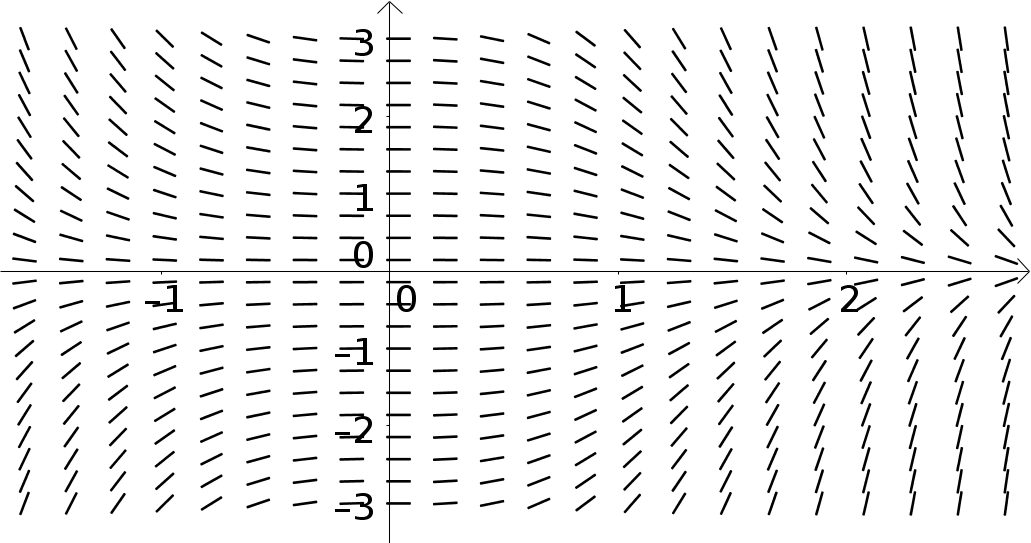
\includegraphics[scale=1]{retn}
	\caption{Tangenten til $ y $ i punktet $ (x, y) $ for kombinasjonene av 31 forskjellige verdier av $ x $ og $ y $. \label{retn}}
\end{figure}
Vi har sett at differensialligninger har uendelig mange løsninger. Ut ifra \fref{retn} ser det ut til at tallverdien til enhver $ y $
\begin{itemize}
	\item avtar forholdsvis kraftig fram til $ x $ nærmer seg ca. $ -1 $ fra negativ side av tallinja.
	\item forblir tilnærmet konstant i området rundt $ x=0 $.
	\item nærmer seg stadig mot 0 for økende verdier av $ x $.
\end{itemize}
Men nå vet vi jo at den generelle løsningen til (\ref{retn0}) er $ y=Ce^{-\frac{1}{3}x^3} $. For å bekrefte vår beskrivelse av oppførselen, kan vi derfor tegne inn grafen til løsningene for $ {C=2} $ og $ {C=-1} $:
\newpage
\begin{figure}
		\centering
	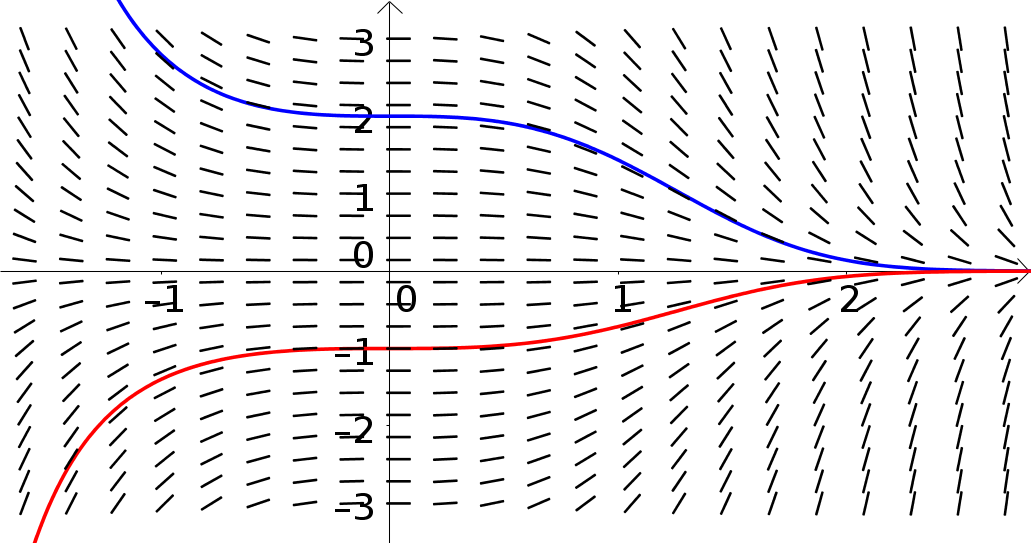
\includegraphics[scale=1]{retn2}
	\caption{Løsningene (integralkurvene) $ {y=2e^{-\frac{1}{3}x^3}} $ (blå) og $ {y=-e^{-\frac{1}{3}x^3}} $ (rød) tegnet inn i retningsdiagrammet.}
\end{figure}
Kurvene til bestemte løsninger av differensialligninger kalles \textit{integralkurver}. \index{integralkurver}
\eks{
Gitt differensialligningen 
\[ x^2y'+3y = 4x \]	
\textbf{a)} Finn et uttrykk for $ y' $. \os
\textbf{b)} Finn stigningstallet til $ y $ i punktene $ (1, 1) $ og $ (-1, 2) $.

\sv
\textbf{a)}\algv{x^2y'&=4x-3y \\
	y' &= \frac{4x-3y}{x^2}
	}
\textbf{b)} Stigningstallet er verdien til $ y' $ i hvert av punktene:\alg{
	y'(1, 1) &= \frac{4\cdot1-3\cdot1}{1^2} \\
	&= 1 \\[5pt]
	y'(-1, 2) &= \frac{4\cdot(-1)-3\cdot2}{(-1)^2} \\
	&= -10 	 
	}
\vds
	}
\newpage
\section[Andre ordens lineære differensialligninger]{Andre ordens lineære differensial- \\ ligninger\label{sode}}
Vi ønsker nå å løse ligningen
\begin{equation}
ay''+by'+cy=0 \label{sodeeq}
\end{equation}
hvor $ a $, $ b $ og $ c $ er konstanter. Dette er en \textit{andre ordens lineær}\index{differensialligning!andre ordens!lineær} differensialligning. Fordi $ y $ og funksjonens deriverte inngår i alle ledd forskjellige fra 0, betegnes den i tillegg som \textit{homogen}\index{homogen}.\vsk

For de lineære ligningene vi så på i \hrs[seksjon]{fode} var eksponentialfuksjonen alltid en del av løsningen. Dette, i tillegg til funksjonens særegne egenskap ved derivasjon, gjør at det er naturlig å sjekke om den er innblandet også her. Vi setter derfor $ {y=e^{rx} }$, for en konstant $ r $, inn i (\ref{sodeeq}). Da får vi at
\begin{align}
	a\left(e^{rx}\right)''+b\left(e^{rx}\right)'+ e^{rx} &= 0\nonumber \\
	ar^2e^{rx}+ bre^{rx} + ce^{rx}&= 0\nonumber\\
	\left(ar^2 + br + c\right)e^{rx} &= 0 \tag{$ e^{rx}\neq 0 $}\nonumber \\
	ar^2 + br + c &= 0 \label{sodkar}
\end{align}
Ligning (\ref{sodeeq}) er derfor oppfylt hvis vi kan finne en $ r $ som oppfyller andregradsligningen over. \eqref{sodkar} kalles den \textit{karakteristiske ligningen}\index{karakteristisk ligning} til \eqref{sodeeq} og kan løses ved \textit{abc-formelen}:
\[ r = \frac{-b\pm\sqrt{b^2-4ac}}{2a} \]
I tidligere skolematematikk har vi sagt at \eqref{sodkar} ikke har en \textit{reell} løsning\footnote{Mange tekster opererer også med at ligningen ikke har noen løsning.}\label{rkmpstart} når  ${ b^2-4ac<0 }$, og stoppet der. Men det viser seg at vi går glipp av mange løsninger av (\ref{sodeeq}) om vi ikke også tar med de \textit{komplekse} løsningene\index{kompleks!løsning} av \eqref{sodkar}.\vsk

I \textit{kompleks analyse} innfører man bokstaven 'i' for å betegne kvadratroten av $( -1) $:
\[ \mathrm{i}=\sqrt{-1} \]
Et tall som $ 3+5\sqrt{-1} $ kalles et \textit{komplekst tall}\index{kompleks!tall}, og skrives gjerne som \\$ 3+5\mathrm{i} $.\vsk

La oss som et eksempel se hvilken konsekvens kompleks analyse har for ligningen
\[ r^2 +9 = 0  \]
Fra ethvert tall kan vi alltid faktorisere ut $ (-1) $, med introduksjonen av 'i' får vi derfor at
\alg{
	r^2 &= -9 \\
	r^2 &= 9(-1) \\
	r &= \pm \sqrt{9(-1)}\\
	&= \pm \sqrt{9}\sqrt{-1}\\
	&= \pm 3\mathrm{i}
	}
Den \textit{komplekse løsningen}\index{kompleks!løsning} er altså $ r=\pm 3\mathrm{i} $.\vsk

Med kjennskapen til komplekse tall er vi klare til å se på alle løsninger av (\ref{sodeeq}):
\sode
\sodee
\sodeeto
\sodeetre
\section{Anvendelser}
Vi skal straks se eksempler på hvordan differensialligninger anvendes i beregninger, men først må vi ha en liten repetisjon av den praktiske tolkningen av derivasjon. Har vi en funksjon $ y(x) $ er $ y' $, kort fortalt, den momentane endringen av størrelsen $ y $ per enhet $ x $. Likeså er $ y'' $ den momentane endringen av størrelsen $ y' $ per enhet $ x $ osv.\vsk

\subsection[$ y '$ proporsjonal med $ y $]{\boldmath $ y '$ proporsjonal med $ y $}
I mange sammenhenger vi finner i naturen studerer vi en størrelse $ y(t) $ som endrer seg med tiden $ t $. I enkelte tilfeller vil vi observere at den momentane endringen per tidsenhet, altså farten\index{fart}, er proporsjonal\index{proporsjonal} med størrelsen selv. Dette betyr at
\[ y' = ky \]
hvor $ k $ er en konstant. Fortegnet til $ k $ avhenger av om $ y $ er voksende ($ k>0 $) eller synkende ($ k<0 $).
\regv
\newpage
\eks[1]{
Hovedprinsippet bak karbondatering\index{karbondatering} (også kalt C-14 metoden) er at alle levende organismer innholder en tilnærmet konstant mengde med den radioaktive isotopen $ {}^{14} $C. Når organismen dør vil derimot innholdet av denne isotopen avta. Ved å sammenligne $ {}^{14} $C-innholdet i en død og en levende organisme av samme art, kan man med god presisjon fastslå alderen til den avdøde organismen. \vsk

For en død organisme er det funnet at endringen i $ {}^{14} $C-mengde per tidsenhet er proporsjonal med mengden $ {}^{14} $C som til enhver tid er i organismen. Hvis vi lar $ y(t) $ være et mål på denne mengden, kan vi skrive
\[ y'=ky \]
hvor $ k $ er en konstant.
Dette er en differensialligning med den generelle løsningen
\[ y = De^{ky} \]
Vi lar $ y $ betegne prosenten av den opprinnelig $ {}^{14} $C-mengde som er igjen i organismen etter $ t $ år. Dette betyr at $ {y(0)=100} $ og dermed at $ D=100 $:
\[ y= 100 e^{ky} \]
\textit{Halveringstiden}\index{halveringstid} til $ {}^{14} $C er 5730 år. Dette betyr at etter så mange år vil $ {}^{14} $C-mengden i en død organisme være halvert. Altså er
\alg{
	y(5730)	&= 50 \\
	100 e^{5730k} &= 50 \\
	5730k &= \ln \frac{1}{2} \br
	k &= \frac{\ln \frac{1}{2}}{5730} \br
	 &\approx -0.000121
	}
For å datere en organisme kan vi derfor bruke funksjonen
\[ y = 100^{-0.000121t} \]\vds
	}
\newpage
\eks[2]{
I en bakteriekultur er økningen i antall bakterier per minutt lik 4\,\% av antallet bakterier. La $ y(t) $ betegne antall bakterier etter $ t $ minutter.\os

\textbf{a)} Sett opp en differensialligning som relaterer $ y' $ til $ y $ og finn den generelle løsningen av denne.\os

\textbf{b)} Sett $ y(0)=1 $. Når vil kulturen inneholde 30 bakterier?

\sv
\textbf{a)}	Differensialligningen blir
\[ y' = 0.04y \]
Dette er en seperabel differensialligning med generell løsning
\[ y = Ce^{0.04t} \]

\textbf{b)} Siden $ {y(0)=1} $, finner vi fort at $ {C=1} $, og derfor at \\$ y=e^{0.04t} $. Vi søker altså en løsning av ligningen
\alg{
 e^{0.04t} &= 30 \br
 t 	&= \frac{\ln 30}{0.04} \br
 &\approx 85.03
	}
Kulturen vil passere 30 bakterier i løpet av det 85. minuttet.

}
\subsection{Populasjonsmodeller}
I en populasjonsmodell\footnote{Navnet populasjon assosieres gjerne med antall mennesker, dyr o.l., men metodene som ligger til grunn for populasjonsmodeller kan like gjerne brukes for å finne utviklingen av mengder som alkohol, medisin osv.} er det spesielt tre faktorer man må ta hensyn til for å beregne en størrelse $ y(x) $:
\begin{itemize}
	\item Hvor mye som, uavhengig av populasjonen, tilføres/fjernes per enhet $ x $.
	\item Hvor stor andel av populasjonen som tilføres per enhet $ x $.
	\item Hvor stor andel av populasjonen som fjernes per enhet $ x $.
\end{itemize}
Siden det er snakk om \textit{endringer per enhet} $ x $, gir punktene over bidrag til uttrykket for $ y' $.\regv
\eks[1]{
Ifølge SSB var netto innvandring\footnote{$\text{antall innvandret} - \text{antall utvandret}$ } til Norge i 2017 talt til 21\,349 mennesker. I tillegg utgjorde antall fødte ca. 1.05\% av folketallet, mens antall døde utgjorde ca. 0.76\% av folketallet. Det totale folketallet var 5\,295\,619\vsk

Anta at netto innvandring per år, prosent fødte per år og prosent døde per år vil være det samme som i 2017 de kommende årene. Sett opp en differensialligning for folketallet $ y(t) $, $ t $ år etter 2017.

\sv \vspace{-7pt}
\begin{itemize}
	\item Netto innvandring per år gir bidraget 21\,349 til $ y' $.
	\item Antall fødte per år gir bidraget  $ 0.0105y $ til $ y' $ .
	\item Antall døde per år gir bidraget  $ -0.0076y $ til $ y' $ .
	\item Siden folketallet var 5\,295\,619 i 2017, er $ y(0)= 5\,295\,619 $.
\end{itemize}
Ligningen blir derfor
\alg{
y' &= 21\,349 + 0.0105y-0.0076y  \\
&= 21\,349+0.0029y
}\vds \vs
} \newpage
\tssec{Fjør-masse-system uten demping}\index{fjør-masse-system!uten demping}
Tenk at vi har en klosse\index{klosse} med masse\index{masse} $ m $ som henger vertikalt i en stiv, masseløs fjør\index{fjør}. Vi plasserer en $ y $-akse vertikalt og definerer nedover som positiv retning.
\begin{figure}
	\centering
	\subfloat[a)]{\includegraphics[]{\asym{fjor1}}}
	\qquad\qquad
	\subfloat[b)]{\includegraphics[]{\asym{fjor}}}
	\caption{\textsl{a)} Fjøra i sin opprinnelige lengde. \textsl{b)} Fjøra og klossen i likevektsstilling. \label{fjorfig}}	
\end{figure}
Når fjøra ikke er påvirket av noen ytre krefter, altså før klossen festes, har den lengden $ L_0 $. Hvis fjøra blir strekt eller komprimert antar vi at fjøra adlyder \textit{Hooks lov}\index{Hooks lov}\footnote{Hooks lov er rimelig å anta så lenge utslaget er mye mindre enn originallengden til fjøra.}. Denne sier at kraften $ F_f $ fra fjøra er proporsjonal med, og motsatt rettet av, forlengelsen/forkortelsen:
\[F_f = -k(L-L_0) \label{fjor}\]
$ k $ er en konstant\index{fjør!-konstant}\footnote{$ k $ har SI-enhet N/m, altså Newton\index{Newton (enhet)} per meter.} bestemt ut ifra fjøras egenskaper, mens $ L $ er den endrede lengden til fjøra. \vsk

Når klossen festes til fjøra, vil tyngdekraften\index{tyngdekraft}\footnote{$ g $ går under navnet \textit{tyngdeakselerasjonen}, verdien tilnærmes ofte til 9.81 m/s$ ^2 $} $ mg $ dra klossen nedover og fjøra strekkes. For en viss fjørlengde $ L_1 $ (se \fref{fjorfig}) vil fjørkraften være like stor, men motsatt rettet av tyngekraften. Dette betyr at
\begin{align}
mg &= -F_f\nonumber	\\
mg &= k(L_1-L_0) \label{likevekt}
\end{align}
Posisjonen festepunktet mellom fjøra og klossen har i dette tilfellet kaller vi \textit{likevektspunktet}\index{likevektspunkt}. Her setter vi $ {y=0} $ (se igjen \fref{fjorfig}). \vsk

\textit{Newtons andre lov}\index{Newtons andre lov} forteller oss at summen av alle krefter $ F_i $ som virker på klossen er lik massen ganger akselerasjonen $ a $:
\[\phantom{testingcloservlo} \sum\limits_{i=1}^n F_i = ma \tag{Newtons andre lov\label{newt2lov}}\]
Tenk nå at vi trekker i klossen slik at festepunktet mellom denne og fjøra blir forskjøvet fra likevektspunktet. Klossen vil da svinge opp og ned. Vi lar $ L(t) $ betegne lengden fjøra har til enhver tid $ t $. Hvis vi ser bort ifra luftmotstand\index{luftmotstand} og all annen form for friksjon\index{friksjon}\footnote{Når friksjonskrefter, altså krefter som alltid motvirker bevegelsen, er neglisjert, sier vi at vi har et system uten demping.}, blir summen av kreftene som virker på klossen følgende:
\alg{
\sum F	&= mg+F_f \\
 &= mg - k(L(t)-L_0)
}
Videre erstatter vi $ mg $ med uttrykket fra (\ref{likevekt}), og anvender \hyperref[newt2lov]{Newtons andre lov}:
\alg{
\sum F &= k(L_1-L_0) - k(L(t)-L_0)	\\
	ma&= -k(L(t)-L_1)
	}
Vi setter  ${y(t)=L(t)-L_1}$. Denne funksjonene beskriver forflytnigen til festepunktet relativt til likevektspunktet $ {y=0} $. Den relative forflytningen til $ y $ samsvarer med den relative forflytningen til massesenteret til klossen. Dette betyr at vi kan erstatte akselerasjonen $ a $ med $ y'' $:
\alg{
my''&= -ky \\
my''+ ky &= 0
	}
\fjmas
\eks{
En klosse med masse $ {m=0.1} $ henger vertikalt i ei fjør med fjørkonstant $ {k=10} $. Klossen forflyttes lengden $ 0.5 $ i positiv retning fra likevektspunktet $ {y=0} $, og blir etterpå sluppet. La $ y(t) $ være forflytningen relativt til likevektspunktet tiden $ t $ etter at bevegelsen har startet.\os

\textbf{a)}  Finn et uttrykk for $ y $.\os

\textbf{b)} Hvor lang tid tar det mellom hver gang klossen er i sitt høyeste punkt?

\sv
\textbf{a)} Vi gjenkjenner dette som et fjør-masse system uten demping, $ y(t) $ er derfor gitt ved ligningen
\[ my''+ky =0 \]
med karateristisk ligning
\alg{
mr^2+k&=0\\
0.1r^2 + 10&=0 \\
r^2 &= \sqrt{-100} \\
&=\pm 10\sqrt{-1} 	
	}
Den generelle løsningen blir derfor (se (\ref{kompleks}))
\[ C \cos(10t)+ D\sin(10 t) \]
Videre vet vi at $ y(0)=0.5 $, som gir oss ligningen
\alg{
C\cos(10\cdot0)+D\sin(10\cdot0) &= 0.5 \\
C &= 0.5
	}
Rett før bevegelsen starter har klossen hastighet 0, noe som betyr at $ y'(0)=0 $:
\alg{
-\frac{C}{10}\sin(10\cdot0) + \frac{D}{10}\cos(10\cdot0)&= 0 \\
D &= 0	
	}
Endelig løsning blir derfor
\[ y = 0.5 \cos(10t)  \]
\textbf{b)} Tiden klossen bruker fra topp tilbake til topp er perioden $ P $ til svingebevegelsen. Denne er gitt som (se (\ref{ker2pioverP}))
\[ P=\frac{2\pi}{10} \]
Det tar klossen $ 0.2\pi $ tidsenheter å fullføre en svingebevegelse.
	}

\tssec{Fjør-masse system med demping}\index{fjør-masse-system!med demping}
Vi har akkurat sett på et fjør-masse system hvor alle friksjonskrefter er neglisjert. Hvis slike krefter derimot tas med i betraktningen, sier vi at systemet er \textit{dempet}\index{demping}. Friksjon er en veldig krevende disiplin innen fysikk, og de matematiske tilnærmingene av fenomenet er mange og varierte. \vsk

Av de enkleste tilnærmingene er å beskrive friksjonen ved størrelsen $ qv $, hvor $ v $ er farten\index{fart} til gjenstanden som ytes motstand og $ q $ er et friksjonstall\index{friksjonstall} med enhet kg/s. Hvis vi tilføyer dette leddet i (\ref{fjormass}), får vi at
\[ my'' + qy'+ky = 0 \]
hvor $ v $ er erstattet med $ y' $.\regv
\fjmasd
\newpage
\eks{
Gitt et fjør-masse system med $ {m=1} $, $ {k=5} $ og $ {q=4} $. Finn forflytningen $ y(t) $ relativt til likevektspunktet når massen initielt blir gitt en forflytning $ {y(0)= 1}$, og deretter sluppet.

\sv
Dette er et fjør-masse system med demping, $ y(t) $ er derfor gitt ved ligningen
\[ my'' + qy'+ky = 0 \]
som har karakteristisk ligning
\alg{
mr^2+qr+k&=0\\
r^2 + 4r + 5 &= 0 \\
r &= \frac{-4\pm\sqrt{4^2-4\cdot5}}{2} 	\br
&= \frac{-4 \pm \sqrt{-4}}{2}\br
&= \frac{-4\pm 2\sqrt{-1}}{2} \br
&= -2 \pm \sqrt{-1}
	}
Den generelle løsningen blir derfor
\[ y=e^{-2t}\left(C\cos t + D \sin t\right) \]
Siden $ y(0)=1 $, får vi at
\alg{
e^{-2\cdot0}\left(C\cos 0 + D \sin 0\right) &= 1 \\
C &= 1	
	}
Videre vet vi at massens hastighet må ha vært 0 idét den ble sluppet, altså at $ y'(0)=0 $:
\alg{
-2e^{-2\cdot0}(C\cos 0+ D\sin 0 )+ e^{-2\cdot0}(-C\sin 0+ D\cos 0 )&= 0 \\
-2 C + D &= 0\\
D &= 2C \\
D &= 2	
	}
Altså er
\[y= e^{-2t}\left(\cos t + 2 \sin t\right) \]\vds
}
\newpage
\tsec{Forklaringer}
\subsection*{Andre ordens differensialligninger}
I \hrs[seksjon]{sode} har vi sett at ligningen
\begin{equation}
ay''+by'+cy = 0 \label{sodeforkl}
\end{equation}
har ${y= e^{rx}} $ som løsning hvis $ r $ oppfyller den karakteristiske ligningen
\begin{equation}
ar^2 + br + c = 0 \label{kar}
\end{equation}
I tillegg ble det nevnt i seksjon \ref{difgen} at vi for disse typen ligninger forventer en generell løsning som består av to konstanter vi ikke kan slå sammen til én. Mer nøyaktig forventer vi at løsningen er en \textit{lineærkombinasjon}\index{lineærkombinasjon} av to \textit{lineært uavhengige}\index{lineært uavhengig} funksjoner, men hverken disse to begrepene eller et bevis for dette skal vi bruke tid på her. Isteden skal vi se noe overfladisk på hvorfor løsningene blir så forskjellige for de tre tilfellene av den karakteristiske ligningen. \vsk

Vi starter med å vise at hvis $ {y=y_1} $ og $ {y=y_2} $ er to løsninger av (\ref{sodeforkl}), så er $ {y=y_1 + y_2 }$ også en løsning:
\alg{
	a(y_1+y_2)''+b(y_1+y_2)'+c(y_1+y_2) &= 0	 \\
	ay_1''+ay_2''+ by_1'+by_2' + cy_1+cy_2 &= 0 \\
	\underbrace{ay_1''+ by_1' + cy_1}_{0}+\underbrace{ay_2''+by_2'+cy_2}_{0} &= 0
}
Med samme framgangsmåte kan vi også vise (prøv selv!) at hvis $ {y=y_1} $ er en løsningen, må $ y=Cy_1 $ også være det. \vsk

Av det som er drøftet over, er målet nå å finne to funksjoner $ y_1 $ og $ y_2 $ som begge oppfyller (\ref{sodeforkl}), og som er slik at $ {y_1\neq Dy_2} $. Da vil nemlig $ {y=Cy_1+Dy_2} $ være den komplette løsningen av differensialligningen.\vsk

\textbf{To reelle røtter}\bs
Når (\ref{kar}) har to distinkte og reelle røtter $ {r=r_1} $ og $ {r=r_2} $, betyr dette at både $ {y_1=e^{r_1x}} $ og $ {y_2=e^{r_2x} }$ er løsninger av (\ref{sodeforkl}). Da må også både $ {y_1=Ce^{r_1x}} $ og $ {y_2=De^{r_2x}}$ være løsninger av differensialligningen. Og fordi $ r_1\neq r_2 $, må vi ha at $ Ce^{r_1 x}\neq De^{r_2 x} $. Den generelle løsningen vi søker er dermed
\[ y=Ce^{r_1}+De^{r_2}   \]
\newpage
\textbf{Én reell rot}\bs
Hvis (\ref{kar}) har én rot $ {r=r_1} $, er $ {y=e^{r_1x}} $ en løsning av \eqref{sodeforkl}. Men om vi som i tilfellet av to reelle røtter legger sammen løsningene ${y_1 =Ce^{r_1x}} $ og ${y_2= De^{r_1x}} $, ender vi opp med løsningen $ {y=(C+D)e^{r_1 x} }$. Dette motstrider det løselig definerte kravet vårt om to konstanter som ikke kan slås sammen til én for å ha en komplett løsning.\vsk

Dette motiverer oss til å søke en løsning på formen $ {y=u(x)e^{r_1x} }$, hvor $ u $ er en ukjent funksjon av $ x $.
Når $ {r=r_1} $ er den eneste løsningen av den karakteristiske ligningen, må denne være på formen
\[ (r-r_1)^2=r^2-2r_1r+r_1^2=0  \]
Dette betyr at differensialligningen kan skrives som
\[ y''-2r_1 y'+r_1^2y=0 \]
Setter vi $ y=u(x)e^{r_1x} $ inn i ligningen over, får vi at
\alg{
	\left(ue^{r_1x}\right)''-2r_1 \left(ue^{r_1x}\right)'+r_1^2ue^{r_1x}&=0 \br
	\left((u'+r_1u)e^{r_1x}\right)'-2r_1(u'+r_1u)e^{r_1x} + r_1^2ue^{r_1x} &=0 \br
	\left((u''+r_1u')+r_1(u'+r_1u)-2r_1(u'+r_1u) + r_1^2u\right)e^{r_1x}&=0 \tag{$ e^{r_1x}\neq0 $}\br
	u''+r_1u'+r_1(u'+r_1u)-2r_1(u'+r_1u) + r_1^2u &=0 \br
	u'' &= 0
}
Ved integrasjon to ganger finner vi at $ u=C+Dx $, og dermed at 
\[ y = (C+Dx)e^{r_1x} \]
\textbf{To komplekse røtter}\bs
Det kan kanskje virke litt rart at alle løsninger av (\ref{sodeforkl}) hittil har bestått av eksponentialfunksjonen\index{eksponentialfunksjon}, mens vi i tilfellet av to komplekse røtter ender opp med en kombinasjon av sinus og cosinus. Men for to komplekse røtter $ {r= p+\mathrm{i}q}$ og $ {r= p-\mathrm{i}q}$ får vi faktisk en generell løsning på akkurat samme formen som for tilfellet av to reelle røtter:
\alg{y &= \hat{C}e^{(p+\mathrm{i}q)x}+\hat{D}e^{(p-\mathrm{i}q)x}\\&=e^{px}(\hat{C}e^{\mathrm{i}qx}+\hat{D}e^{-\mathrm{i}qx}) }
Til forskjell tillates her komplekse verdier\index{kompleks!verdi} også for de vilkårlige konstantene, noe som er indikert ved symbolet '$ \;\hat{}\; $'. Men skal differensialligningen brukes til å modellere fysiske systemer fra virkeligheten, må vi sørge for at løsningen er reell. For å utrette dette anvender vi \textit{Eulers formel}:
\[ \phantom{aaaaaa}e^{\mathrm{i}qx}=\cos(qx)+\mathrm{i}\sin(qx) \tag{\text{Eulers formel}}\]
Av denne kan vi skrive (husk at $ {\cos(-x)=\cos x} $ og at $ {\sin(-x)=-\sin x} $)
\small \alg{
\hat{C}e^{\mathrm{i}qx}+\hat{D}e^{-\mathrm{i}qx} &= \hat{C}(\cos(qx)+\mathrm{i}\sin(qx))+ \hat{D}(\cos(-qx)+\mathrm{i}\sin(-qx))	\\
&= (\hat{C}+\hat{D})\cos(qx)+\mathrm{i}(\hat{C}-\hat{D})\sin(qx)
	}
\normalsize
Ved riktig valg\footnote{Vi lar $ \hat{C}=a+\mathrm{i}b $ og $ \hat{D}=a-\mathrm{i}b $, hvor $ a $ og $ b $ er to reelle konstanter.} av $ \hat{C} $ og $ \hat{D} $ kan vi lage oss de reelle tallene $ {C=\hat{C}+\hat{D}}  $ og $ D=\hat{C}-\hat{D} $, og med det få den reelle løsningen
\[ y =  e^{px}(Ccos (qx) + D \sin (qx))  \]
\end{document}
